\section{Feigenbaum's Theory of Scaling}

The whole theory of bifurcation is spectacular; even more amazing are the Feigenbaum constants $\alpha$ and $\delta$, whose existence and universality are demonstrated by the numerics in Tables \ref{tab:feigenbuam_alpha_table_for_logistic} and \ref{tab:feigenbuam_constants_skewed_logistic_map}. 
The existence of universal constants across a wide class of chaotic dynamical systems is a quintessential quantifiable property of chaos.
The proof that these constants exist and are universal is well beyond the scope of this undergraduate project, but we can give some rational argument as to the existence of $\alpha$.

\begin{figure}
    \centering
    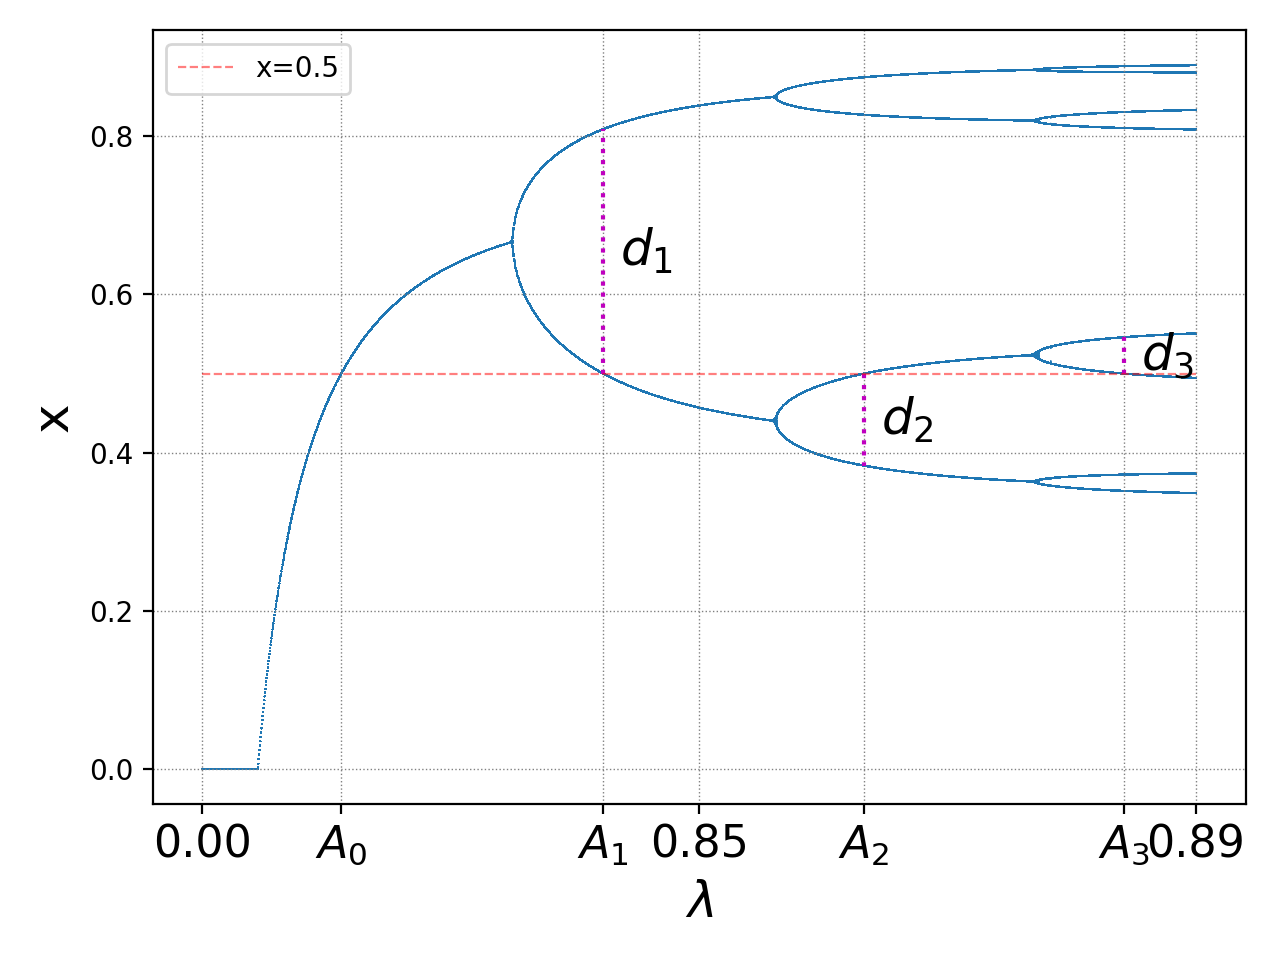
\includegraphics[width=0.6\linewidth]{Images/demonstration of feigenbaum constants.png}
    \caption{Bifurcation diagram of the logistic map, which shows the location of four parameter values $A_n$ which correspond to where each $2^n$ cycle achieves superstability. The distances $d_{n+1}$ are those between $X_m$ and the closest point in the cycle.}
	\label{fig:universal_raito}
\end{figure} 

For a given iterative map $F$ depending on one parameter satisfying the requirement of Theorem \ref{th:criteria_for_infinite_bifurcations}, $d_i$ is the distance at the superstability of the $2^{i}$ cycle between $X_{m}$ and its closest point in the cycle, where $X_m$ is the unique maximum of $F$.

Recall that $\alpha = \lim_{i \rightarrow  \infty}\frac{b_i}{b_{i-1}}$. 
Writing it in another way
\begin{equation}\label{eq:d_sim}
d_r \sim\frac{D}{(-\alpha)^r} \quad \quad \text{ as } r \to \infty
\end{equation}
where $D$ is a constant depending on $F$ and $\alpha$ is Feigenbaum's $x$-scale constant. 

Theorem \ref{th:logistic_bifurcation}.\ref{log_closest_branch} states that $d_i = F^{2^{n-1}}(A_i, X_m) - X_m$, where $A_i$ is the value of the parameter at which the $2^n$ cycle achieves superstability and crosses $X_m$. An example of these distances is shown in Figure \ref{fig:universal_raito}.
Therefore, to find the scaling of $d_r$, we take the limit of \eqref{eq:d_sim},

\begin{equation}
\lim_{r \to \infty} (-\alpha)^r \left(F^{2^r}(A_{r+1}, X_m) - X_m\right) = - D/\alpha.
\end{equation}

This leads to the hypothesis that
$$
g_1(x-X_m)=\lim_{r \to \infty} \{g_{1r}(x-X_m)\},
$$
where
$$
g_{1r}(x-X_m) = (-\alpha)^r \{F^{2r}(A_{r+1}, X_m + (x-X_m)/(-\alpha)^r)-X_m\}.
$$
Let $x-X_m$ be the difference from the point of superstability about the bifurcation to $X_m$. 
From the scaling of $d_r$, this implies that $g_1(0)=-\frac{D}{\alpha}$ and by solving for the first couple of iterations of $g_{1r}(x-X_m)$, we can see a limit emerges for $g_1$.
Feigenbaum believed that $g_1$ is dependent on the scaling of $x-X_m$ which shows the behaviour of $F$ near to its maximum. 
% Since $g_1$ doesn't matter on the map $F$ we can thus say that this behaviour causes $g_1$ to become universal.

Without loss of any generality we can set $X_m=0$.
The main ideas of scaling $x$ can be seen by the operator $T$, which we define to be
\begin{equation} \label{eq: operator T}
T\psi(x)=-\alpha \psi (\psi(-\frac{x}{\alpha})).
\end{equation}
Setting $\psi=g_1$, we have
\begin{align}
    Tg_1 &=-\alpha g_1(g_1(-x/\alpha)) \nonumber \\
    &= -\alpha \lim_{r \to \infty} \{(-\alpha)^rF^{2r}(A_{r+1}, (-\alpha)^rF^{2r}(A_{r+1},x/(-\alpha)^{r+1}))\}.  \label{eq:one}
\end{align}
Now, if we set $\phi(y)=(-\alpha)^rF^{2r}(A_{r+1},y/(-\alpha)^r))\}$ such that $$\phi^2=\phi(\phi(y))=(-\alpha)^rF^{2r+1}(A_{r+1},y/(-\alpha)^r))\}$$ and $y=\frac{x}{\alpha}$, we can see that
\begin{align*}
    Tg_1 &= \lim_{r \to \infty} \{(-\alpha)^{r+1}F^{2r+1}(A_{r+1}, x/(-\alpha)^{r+1})\} \\
    &= \lim_{q \to \infty} \{(-\alpha)^qF^{2q}(A_q,x/(-\alpha)^q)\} \\
    &= g_0(x)
\end{align*}
This then implies that $Tg_k(x)=g_{k-1}(x)$ for $k = 2,3,...$ where we have shown that,
\begin{align}
    g_k=\lim_{r \to \infty} \{(-\alpha)^{r}F^{2r}(A_{r+k}, x/(-\alpha)^{r})\}. \label{eq:two}
\end{align} 
We can now take the limit as $k \to \infty$ to show that there exists a function $g(x)= \lim_{k \to \infty}g_k(x)$ such that  the functional equation
\begin{align}
    Tg=g \label{eq:FunctionalOperator}
\end{align}
holds. 
And $g$ is a `fixed point' of the nonlinear functional operator $T$.

Using the functional equation \eqref{eq:FunctionalOperator}, the constant $\alpha$ must be determined as part of the solution. 
The function $g(x)$ satisfies this functional equation, and it possesses a scaling symmetry, such that if $g(x)$ is a solution, then the rescaled function $\mu g(x/\mu)$ is also a solution for any $\mu \neq 0$. 
This scaling symmetry implies that there is an inherent freedom in the choice of the parameter $\mu$.
By convention, $\mu$ is chosen such that 
$$
g(0)=1.
$$
Setting $x=0$ in the functional equation, we have, by the original definition  of our operator,
\begin{equation}\label{eq:alpha}
\alpha = -1/g(1).
\end{equation}

Feigenbaum was able to numerically verify the method, where he found that
\begin{align}
    g(x)= 1 - 1.52763x^2 + 0.10482x^4- 0.02671x^6 + \dots .\label{eq:feigenbaum}
\end{align}
This corresponds to the desired $\alpha =-1/g(1)=2.5029$.

\begin{exmp} The Logistic Map
	The logistic map, defined by $F(a,x)=ax(1-x)$, attains its maximum value at $X_m =1/2$.
	Thus we are able to replace $x-X_m$ with $x-1/2$. Hence our new function is given as $F(a,x)=a(1/4-x^2)-1/2$, ensuring that the maximum value of our new function occurs at $x=0$. Using equations \eqref{eq:one} and \eqref{eq:two} we can now see that,
    \begin{align}
        g_{10}&=F(A_1,x)=A_1(1/4-x^2)-1/2 \nonumber \\
        g_{11}&=(-\alpha)F^2(A_2,x/(-\alpha)) \nonumber \\
        &= \alpha A_2 \left(\left(A_2 \left(x^{2}/\alpha^2 - 1/4\right) + 1/2\right)^{2} - 1/4\right) + \alpha/2
    \end{align}
    Thus, for $g_{1r}(x)$, we can plot our findings as $r \to \infty$ in the $x, y$ plane where $y=g_{1r}(x)$. 
	When we present our first couple of plots, we can see a clear limiting function $g_{k=1}$ appearing as $r$ increases. Thus from \eqref{eq:two} we can see that, as we increase $k$, the sequence of functions converges to some function $g(x)$. 
	This is demonstrated in Figure \ref{fig:unscaled}.
	\begin{figure}
    \centering    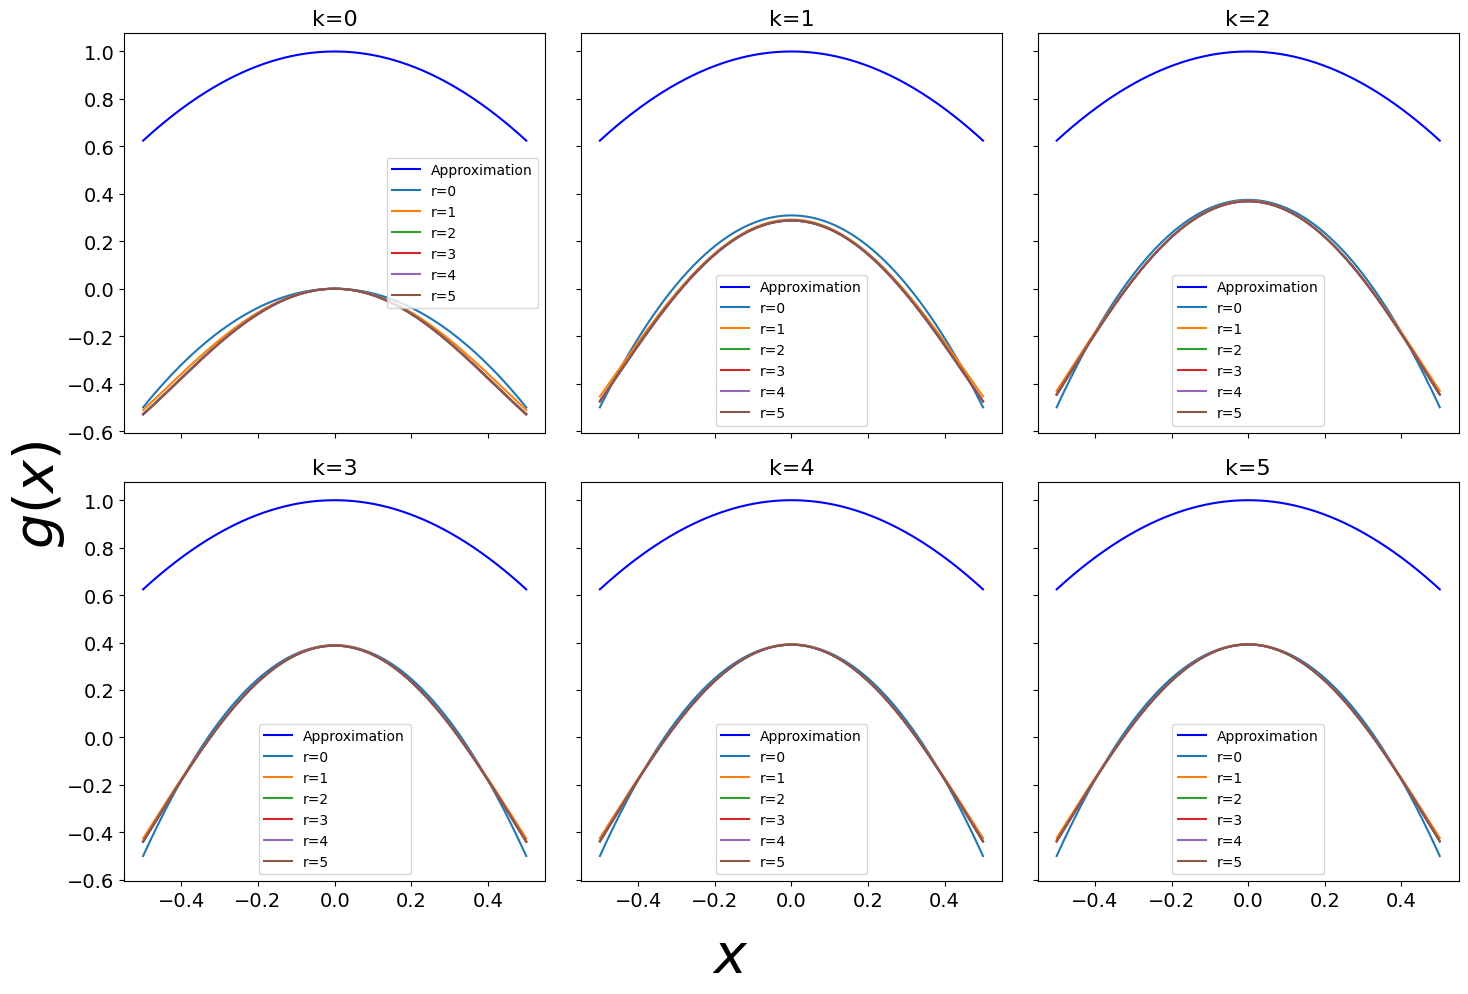
\includegraphics[width=1\textwidth]{Feigenbaum Approx Graphs/feignabum.png}
    \caption{Unscaled graphs corresponding to the logistic map showing the convergence to a limiting function as we iterate over $r,k$. The lines don't converge to Feigenbaum's results meaning that there must exist a scaling factor $\mu$ which needs to be applied.}
    \label{fig:unscaled}
\end{figure}
    

    The blue line in Figure \ref{fig:unscaled} shows us Feigenbaum's numerically solved solution \eqref{eq:feigenbaum} while the rest of the lines show us the iterations of $r$ for specified $k$ values. 
	By iterating $r$ the function seems to converge to some limit, which, however, is different from the solution of Feigenbuam.
	This issue can be resolved by rescaling the function $g(x)$ by an appropriate factor $\mu = \frac{1}{g(0)}$, where $g(0)$ here is our map's solved unscaled value at 0. 
    From our findings, we found that our value of $g(0)$ is $0.39176186028018406$ such that the corresponding scaling factor was found to be $\mu= 2.552571093277968$. Now that we have our new rescaled function $g(x)$, we can plot the iterations of $r$ and $k$. 
	The results are shown in Figure \ref{fig:rescaled}.
    \begin{figure}
    \centering
    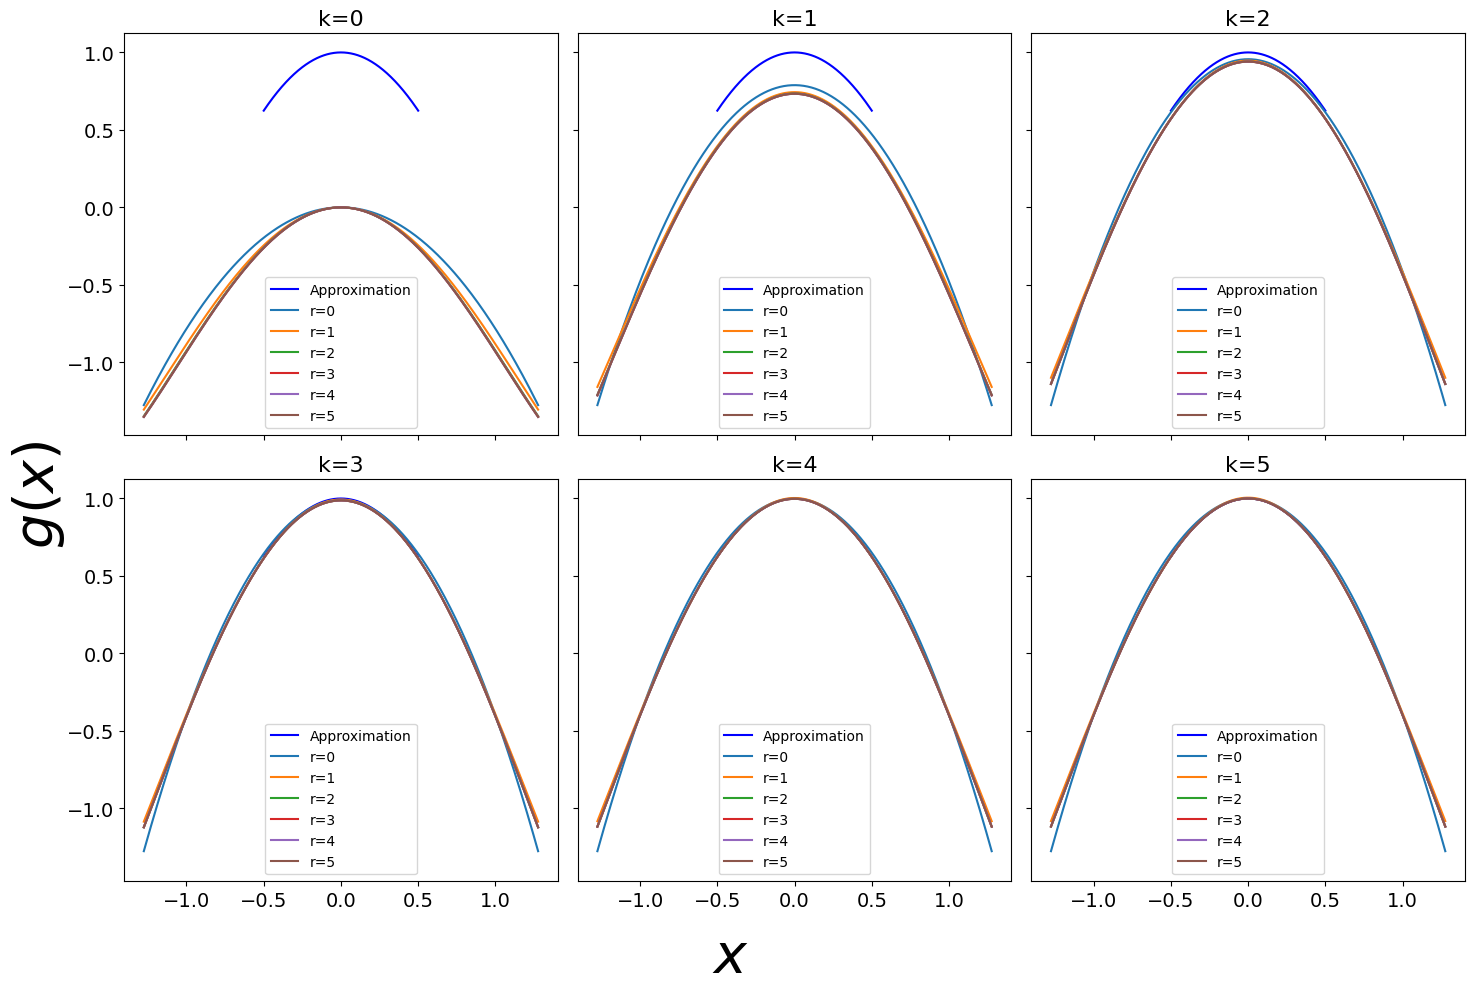
\includegraphics[width=1\textwidth]{Feigenbaum Approx Graphs/feigenbaum_scaled.png}
    \caption{Rescaled graphs with scaling factor $\mu=2.552571093277968$, corresponding to the logistic map which shows the convergence to the limiting function as we iterate $r,k$ that aligns Feigenbaum's numerics.}
    \label{fig:rescaled}
\end{figure}
The blue lines again show us Feigenbaum's numerically solved solution \eqref{eq:feigenbaum}. 
We can now see that due to $\mu$, our rescaled $g(x)$ now shifts up towards Feigenbaum's solution and attains the desired shape showing us that we have successfully rescaled our original solution to the universal one presented by Feigenbaum. 
Thus we have demonstrated the convergence described by Feigenbaum towards his numerical solution as well as the existence of a limiting function $g(x)$ as we increase both $r$ and $k$ simultaneously. 
\end{exmp}

\section{Numerical Computation of Eigenfunction of $T$}

To make the above section rigorous, and to prove the existence of an eigenfunction of the operator $T$, is non-trivial and requires a hundred-page proof \cite{lyubich1999feigenbaum}, let alone finding such a function, and is clearly out of the scope of an undergraduate mathematical report like this one. 
In this section, we will attempt to compute the first few terms of the power series of this eigenfunction.

Assuming $g(0) = 1$ and that $g$ is an even function, (the validity of such assumption is justified by the fact that a successful result was found based on it), it can be written in the form of Taylor expansion 
$$
g = 1 + b_1 x^2 + b_2x^4 + \cdots 
$$
Defining the $n$th partial sum of this power series as $g = 1 + b_1x^2 + \cdots + b_{n-1}x^{2n-2}$, and applying $T$ to $g_n$ will produce another $(2n-2)^2$-degree polynomial whose coefficients depend on $b_1, \cdots, b_{n-1}$, and $\alpha$.
Ignoring the terms of degree higher than $2n-2$, and equating the coefficients of the result with that of $g$ of the same degree will give $n$ functions for $n$ variables, whose solution can be solved numerically. 

We will demonstrate an example for $g_1 = 1 + b_1 x^2$. 

Note 
$$
g_1\left(-\frac{x}{\alpha}\right) = 1 + b_1 \frac{x^2}{\alpha ^2}
$$

and, by plugging in,

\begin{align*}
-\alpha g_1\left(g\left(-\frac{x}{\alpha}\right)\right) 
&= -\alpha\left( 1 + b_1\left(1+b_1 \frac{x^2}{\alpha^2}\right)^2\right) \\
&= -\alpha\left(1 + b_1\left(1 + b_1^2\frac{x^4}{\alpha^4} + x^2 \frac{2b_1}{\alpha^2}\right)\right) \\
&= -\alpha (1 + b_1)  - \frac{2b_1^2}{\alpha} x^2 - \frac{b_1^3}{\alpha^3}x^4
\end{align*}

thereby comes the equation 

$$
\begin{cases}
    1 &= -\alpha(1+b_1) \\
    b_1 &= -\frac{2b_1^2}{\alpha} 
\end{cases}
$$

The solution is $\alpha = 1 + \sqrt{3} \approx 2.732$ and $b_1 = - \frac{\sqrt{3}}{2} - \frac{1}{2} \approx -1.366$.

Calculating any more terms by hand would be an extremely tedious process; luckily, we can resort to computer algebra systems for symbolic manipulation (we used Sympy) and BLAS library (fsolve from Scipy) for solving equations of $n$ variables. 
The approximation for the fifteen terms is shown in Table \ref{tb:b_i table}.
The python code for producing these results is included in Appendix \ref{fsolve}.

By this calculation, and using Equation \eqref{eq:alpha}, an estimation of $\alpha$ is obtained to be $2.5029078754977733823$. We are satisfied with this result as it follows closely to Feigenbaum's own result, implying that our method was successful. Being able to find this constant within a chaotic dynamical system is truly fascinating and a true achievement of Feigenbaum. 

\begin{table}
\centering
\begin{tabular}{|c|c|}
\hline
$n$ & $b_n$ \\
\hline
1 & \( -1.527632997 \times 10^{0} \) \\
2 & \( 1.048151948 \times 10^{-1} \) \\
3 & \( 2.670567058 \times 10^{-2} \) \\
4 & \( -3.527409767 \times 10^{-3} \) \\
5 & \( 8.160111810 \times 10^{-5} \) \\
6 & \( 2.528490972 \times 10^{-5} \) \\
7 & \( -2.556150238 \times 10^{-6} \) \\
8 & \( -9.664817874 \times 10^{-8} \) \\
9 & \( 2.828824961 \times 10^{-8} \) \\
10 & \( -3.352250769 \times 10^{-10} \) \\
11 & \( -2.716117768 \times 10^{-10} \) \\
12 & \( 1.171671302 \times 10^{-11} \) \\
13 & \( 7.447301044 \times 10^{-12} \) \\
14 & \( -2.868216370 \times 10^{-12} \) \\
15 & \( 9.052335129 \times 10^{-13} \) \\
\hline
\end{tabular}
\caption{The values of $b_n$ are the coefficients of the Taylor expression of $g$ such that $g = 1 + \sum_{i=1}^n b_i x^{2i}$, where $g$ is the solution to $Tg = g$.
}
\label{tb:b_i table}
\end{table}


